% !TeX root = ../main.tex
\section{The Rules Through Images}
\label{sec:rules}

This section presents the rules through \emph{screenshots of the software}
rather than formulas, enough for a
non-mathematical reader to grasp the whole game; the corresponding formal
mathematical specification (2-player mode) is in
Appendix~\ref{app:formal}. Convention: \textbf{Green} pieces are drawn in
green and \textbf{Yellow} pieces in yellow; \emph{vertex} pieces sit on the
intersections of the square grid, while \emph{centre} pieces sit between
four vertices. All markers in the images are drawn by the software: a
\emph{yellow ring} marks the selected piece, \emph{green dots} are the
valid landing cells, and \emph{yellow lines} indicate the sandwich ray
from the landing cell. The notation $\mathrm G@(x,y)$ denotes a Green piece
on cell $(x,y)$, and $\mathrm Y@(x,y)$ a Yellow piece.

\subsection{The board---41 cells on two layers}
\label{ssec:vis_board}

\begin{figure}[H]
  \centering
  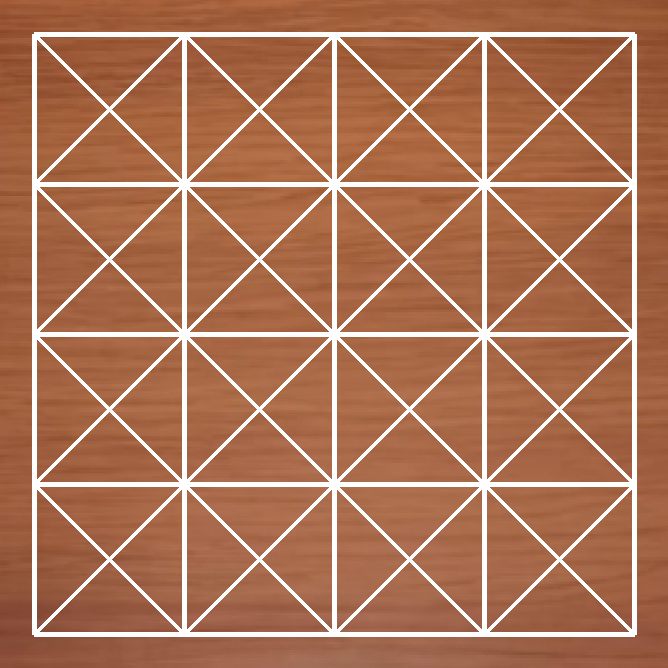
\includegraphics[width=0.5\linewidth]{figures/board_2p_empty.png}
  \caption{Structure of the 2-player board (screenshot of the software,
  the game): 25 \textbf{vertex} cells (intersections of the square grid,
  with integer coordinates such as $(0,0),(2,3)$) plus 16 \textbf{centre}
  cells (intersections of the diagonals, with half-integer coordinates such
  as $(0.5,0.5)$), each centre cell lying exactly in the middle of four
  vertex cells. 41 cells in total. Vertex and centre pieces operate on two
  separate layers that interlock through the diagonals.}
  \label{fig:board41}
\end{figure}

\begin{table}[H]
  \centering
  \caption{Board size and configuration by game mode (exact coordinates and
  starting positions for 3--4 players in
  Appendix~\ref{app:multistart}).}
  \label{tab:board_size}
  \begin{tabular}{lcccc}
    \toprule
    \textbf{Mode} & \textbf{Size} & \textbf{Coordinates}
    & \textbf{Removed cells} & \textbf{Pieces/player} \\
    \midrule
    2-player & 5{\texttimes}5 vertex & $0\text{--}4 \times 0\text{--}4$ & 0 & 14 \\
    3-player & 7{\texttimes}6 vertex & $0\text{--}6 \times 0\text{--}5$ & 4 & 13/13/14 \\
    4-player & 7{\texttimes}7 vertex & $0\text{--}6 \times 0\text{--}6$ & 8 & 13 \\
    \bottomrule
  \end{tabular}
\end{table}

\subsection{Starting position---state 0}
\label{ssec:vis_start}

\begin{figure}[H]
  \centering
  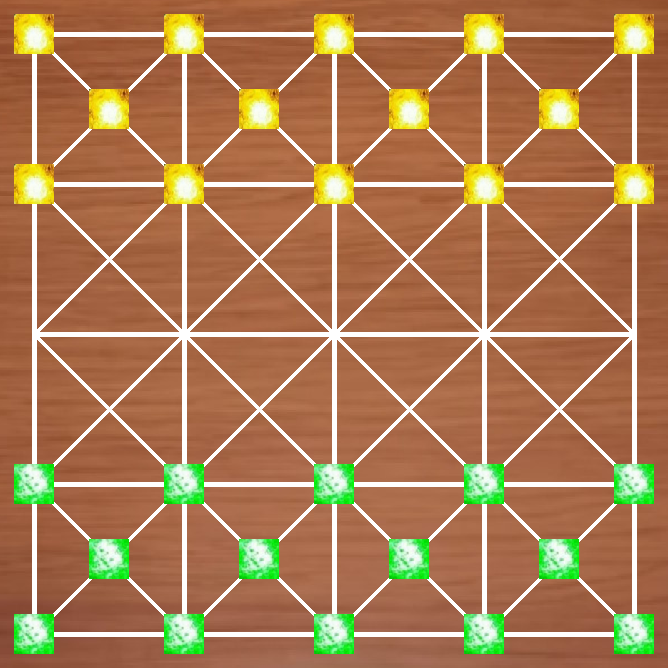
\includegraphics[width=0.5\linewidth]{figures/board_2p.png}
  \caption{The 28 pieces at the starting position (screenshot of the
  software): Yellow and Green, 14 pieces each ($=10$ vertex
  $+\,4$ centre), occupying two rows on opposite sides of the board; the
  three middle rows are empty. Compare
  Equations~\eqref{eq:starty}--\eqref{eq:startg}.}
  \label{fig:start}
\end{figure}

\subsection{Directions---which way pieces move}
\label{ssec:vis_dirs}

\begin{figure}[H]
  \centering
  \begin{subfigure}[b]{0.46\linewidth}\centering
    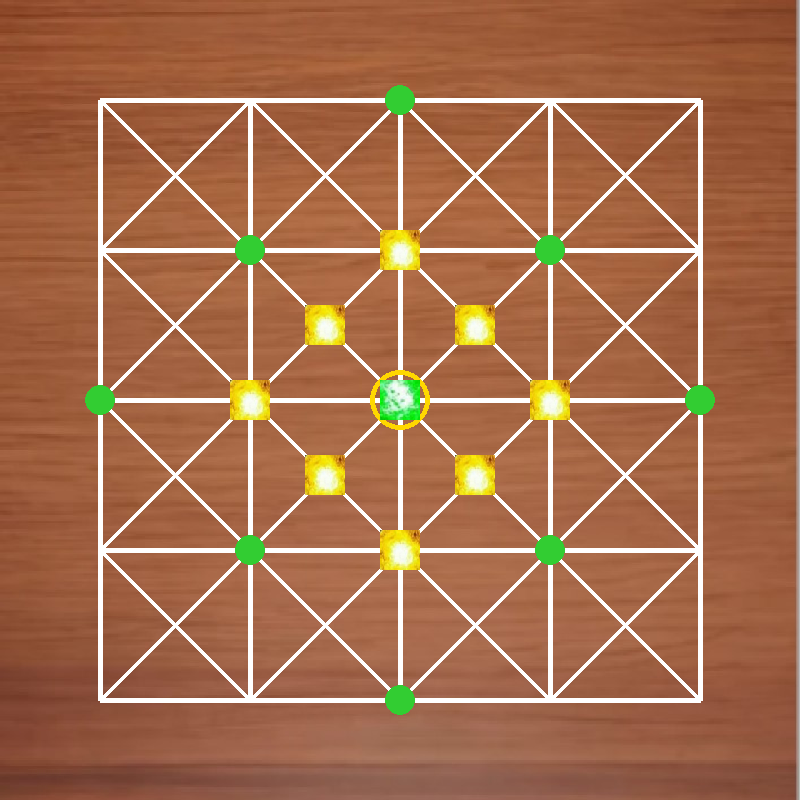
\includegraphics[height=3.4cm]{figures/dir_vertex.png}
    \caption{\textbf{Vertex} piece---8 directions: 4 orthogonal (step 1,
    through an adjacent vertex cell) $+$ 4 diagonal (step $\tfrac12$,
    through a centre cell).}
  \end{subfigure}\hfill
  \begin{subfigure}[b]{0.46\linewidth}\centering
    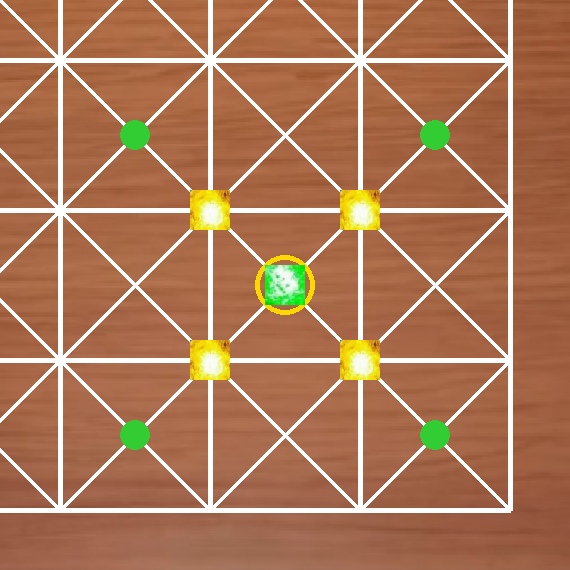
\includegraphics[height=3.4cm]{figures/dir_center.png}
    \caption{\textbf{Centre} piece---only 4 diagonal directions (each step
    through an adjacent vertex cell). Moving orthogonally would fall off
    the centre layer.}
  \end{subfigure}
  \caption{The directions of movement (screenshots of the software; the
  selected piece carries a yellow ring, and the \emph{green dots} are the
  valid landing cells drawn by the software), corresponding to the sets
  $D_{\mathsf V}$ and $D_{\mathsf C}$ in~\eqref{eq:dirs}.}
  \label{fig:dirs}
\end{figure}

\subsection{The jump---the only way to move}
\label{ssec:vis_jump}

A piece moves \emph{only} by jumping: it flies over an adjacent occupied
cell that serves as a \emph{springboard} (of any colour) and lands on the
empty cell immediately beyond it; the springboard piece stays put.
Figure~\ref{fig:jumps} illustrates three kinds of jump.

\begin{figure}[H]
  \centering
  % Example 1: vertex jumps orthogonally
  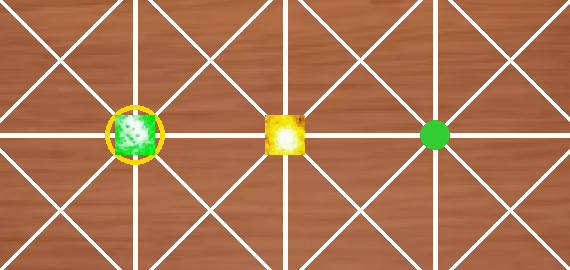
\includegraphics[height=1.9cm]{figures/jump1_before.png}\;$\rightarrow$\;%
  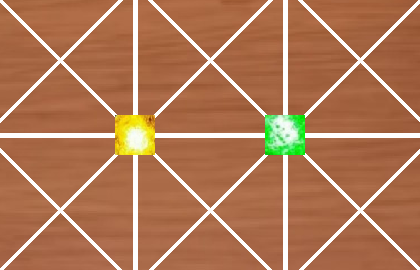
\includegraphics[height=1.9cm]{figures/jump1_after.png}
  \\[0.6em]
  % Example 2: vertex jumps diagonally
  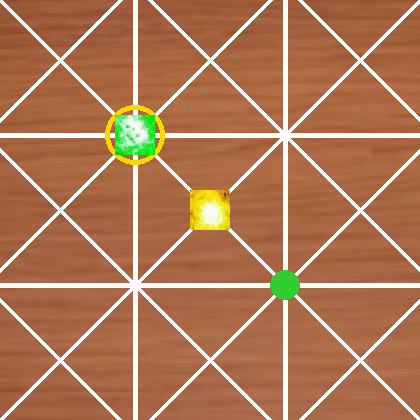
\includegraphics[height=2.3cm]{figures/jump2_before.png}\;$\rightarrow$\;%
  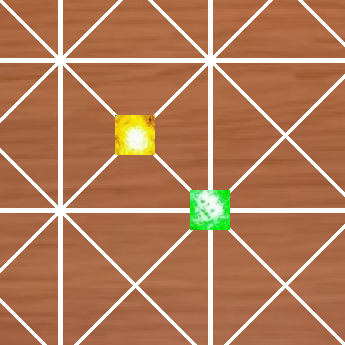
\includegraphics[height=2.3cm]{figures/jump2_after.png}
  \\[0.6em]
  % Example 3: centre jumps diagonally
  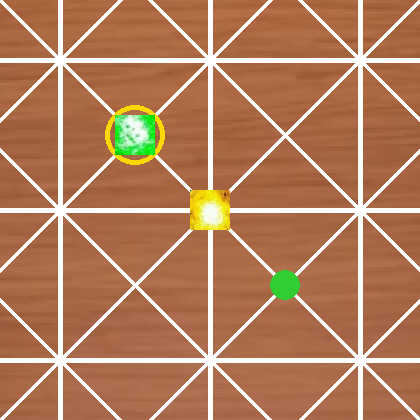
\includegraphics[height=2.3cm]{figures/jump3_before.png}\;$\rightarrow$\;%
  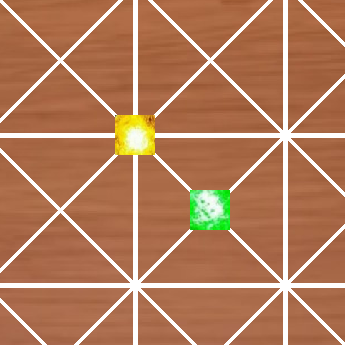
\includegraphics[height=2.3cm]{figures/jump3_after.png}
  \caption{Three jump examples (screenshots of the software, before
  $\rightarrow$ after; yellow ring = selected piece, green dots = valid
  landing cells). \textbf{Top:} a vertex piece jumps orthogonally over the
  springboard $(2,2)$ and lands on $(3,2)$. \textbf{Middle:} a vertex piece
  jumps diagonally using the \emph{centre} cell $(1.5,1.5)$ as springboard
  and lands on the vertex cell $(2,2)$. \textbf{Bottom:} a centre piece
  jumps diagonally using the \emph{vertex} cell $(2,2)$ as springboard and
  lands on the centre cell $(2.5,2.5)$. The springboard always stays in
  place and does not change side.}
  \label{fig:jumps}
\end{figure}

\subsection{Capturing---sandwich and flip}
\label{ssec:vis_capture}

Capture is checked from the landing cell: along each
direction, a run of consecutive opponent pieces immediately followed by one
of your own pieces is sandwiched and changes side.
Figure~\ref{fig:capture} shows a situation with \emph{two} capturing
directions; Table~\ref{tab:capture_rays} lists the details.

\begin{figure}[H]
  \centering
  \begin{subfigure}[b]{0.42\linewidth}\centering
    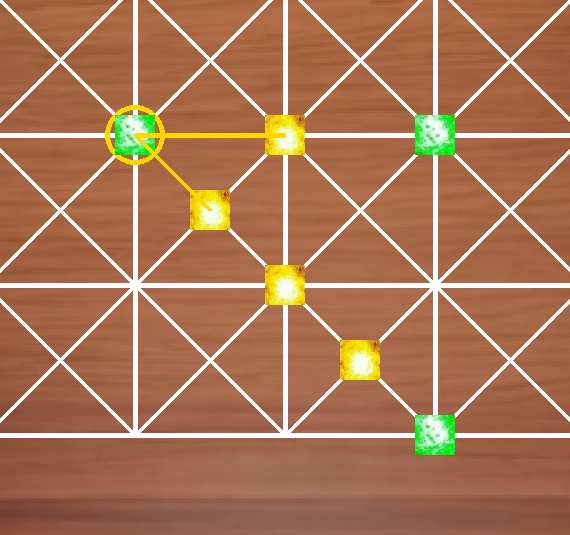
\includegraphics[height=4cm]{figures/capture_before.png}
    \caption{Just landed on $(1,2)$: the game highlights \emph{two}
    capturing rays (yellow).}
  \end{subfigure}\hfill
  \begin{subfigure}[b]{0.42\linewidth}\centering
    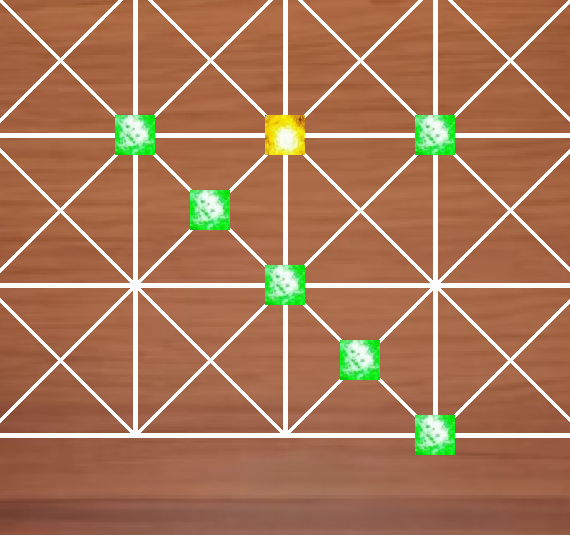
\includegraphics[height=4cm]{figures/capture_after.png}
    \caption{After choosing the diagonal ray and flipping (3 pieces).}
  \end{subfigure}
  \caption{A Green piece has just landed on $(1,2)$ (screenshot of the
  game). There are two capturing directions; the mover chooses
  \emph{one}. Choosing the diagonal ray: the three Yellow pieces
  $(1.5,2.5),(2,3),(2.5,3.5)$ turn Green, while $Y@(2,2)$ on the horizontal
  ray \emph{stays Yellow}---a direction that is not chosen does not flip.}
  \label{fig:capture}
\end{figure}

\begin{table}[H]
  \centering
  \caption{The two capturing directions from landing cell $(1,2)$ in
  Figure~\ref{fig:capture}.}
  \label{tab:capture_rays}
  \setlength{\tabcolsep}{4pt}
  {\small
  \begin{tabular}{lll}
    \toprule
    \textbf{Direction} & \textbf{Ray passes through} & \textbf{Pieces sandwiched} \\
    \midrule
    Horizontal $(1,0)$ & $(2,2){=}\mathrm Y \to (3,2){=}\mathrm G$ & \textbf{1} \\
    Diagonal $(\tfrac12,\tfrac12)$
      & $(1.5,2.5){=}\mathrm y \to (2,3){=}\mathrm Y \to (2.5,3.5){=}\mathrm y \to (3,4){=}\mathrm G$
      & \textbf{3} (2 centre $+$ 1 vertex) \\
    Other directions & broken (hits an empty cell or leaves the board) & 0 \\
    \bottomrule
  \end{tabular}}
\end{table}

\noindent\textbf{Selection rule:} if a sandwich exists you \emph{must}
capture, and you choose exactly \emph{one} direction. Choosing the
direction that captures the most is merely a tactic, not a rule; a player
may capture fewer pieces in order to set a trap.

\subsection{How a move unfolds---three steps}
\label{ssec:vis_move}

\begin{figure}[H]
  \centering
  \begin{subfigure}[b]{0.32\linewidth}\centering
    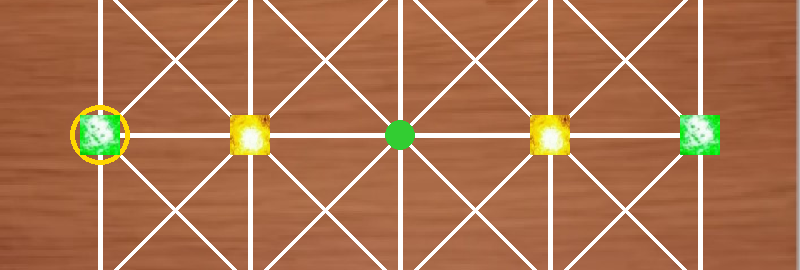
\includegraphics[width=\linewidth]{figures/move_a.png}
    \caption{A. Before the jump.}
  \end{subfigure}\hfill
  \begin{subfigure}[b]{0.32\linewidth}\centering
    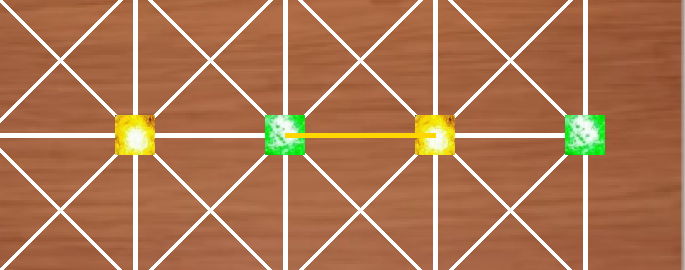
\includegraphics[width=\linewidth]{figures/move_b.png}
    \caption{B. After the jump, before flipping.}
  \end{subfigure}\hfill
  \begin{subfigure}[b]{0.32\linewidth}\centering
    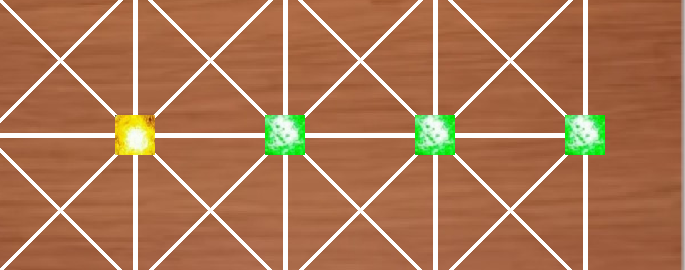
\includegraphics[width=\linewidth]{figures/move_c.png}
    \caption{C. After flipping, turn passes.}
  \end{subfigure}
  \caption{One complete move (screenshots of the software). (A) $G@(0,2)$
  jumps over the springboard $Y@(1,2)$ and lands on $(2,2)$. (B) the
  rightward ray sandwiches $Y@(3,2)$ between the piece that just landed and
  $G@(4,2)$. (C) $Y@(3,2)$ turns Green; the springboard $Y@(1,2)$
  \emph{stays Yellow}; it is now Yellow's turn. The three steps correspond
  to~\eqref{eq:t1}--\eqref{eq:t3}.}
  \label{fig:fullmove}
\end{figure}

\subsection{Turn order}
\label{ssec:turn_order}

Who moves first is agreed among the players; after that the sides move in
turn around the board, one move per turn. The software fixes one clockwise
order: in the 2-player mode Green moves first; in the 3-player mode the
order is Purple $\to$ Yellow $\to$ Green; in the 4-player mode it is
Blue $\to$ Green $\to$ Purple $\to$ Yellow.

\subsection{When the game ends}
\label{ssec:vis_end}

In the 2-player mode, when it is a side's turn and that side has no piece
able to jump, it loses immediately (condition~\eqref{eq:terminal}); the
3--4 player modes are covered in Section~\ref{ssec:elimination}. There are two ways to lose,
shown in Figure~\ref{fig:endgame}.

\begin{figure}[H]
  \centering
  \begin{subfigure}[b]{0.46\linewidth}\centering
    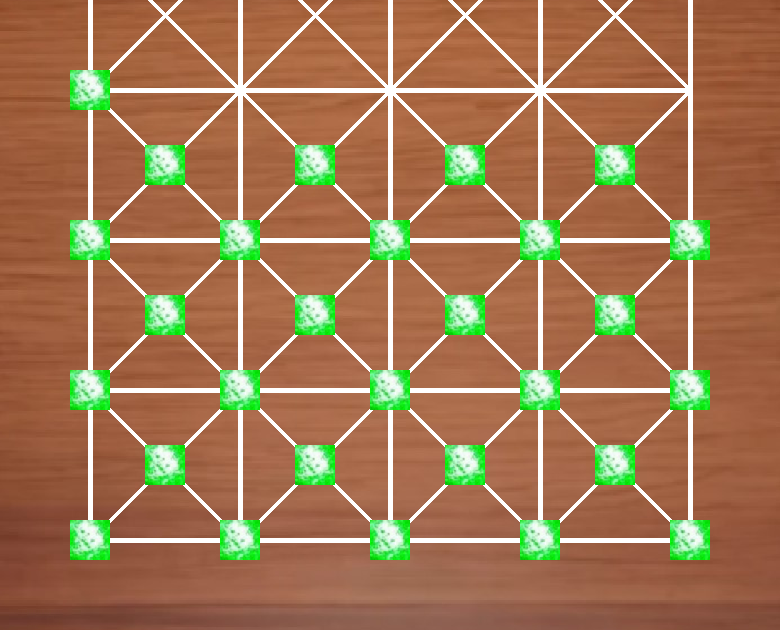
\includegraphics[height=4.2cm]{figures/end_nopieces.png}
    \caption{Out of pieces: all 28 pieces now belong to Green; Yellow has
    nothing left to move.}
  \end{subfigure}\hfill
  \begin{subfigure}[b]{0.46\linewidth}\centering
    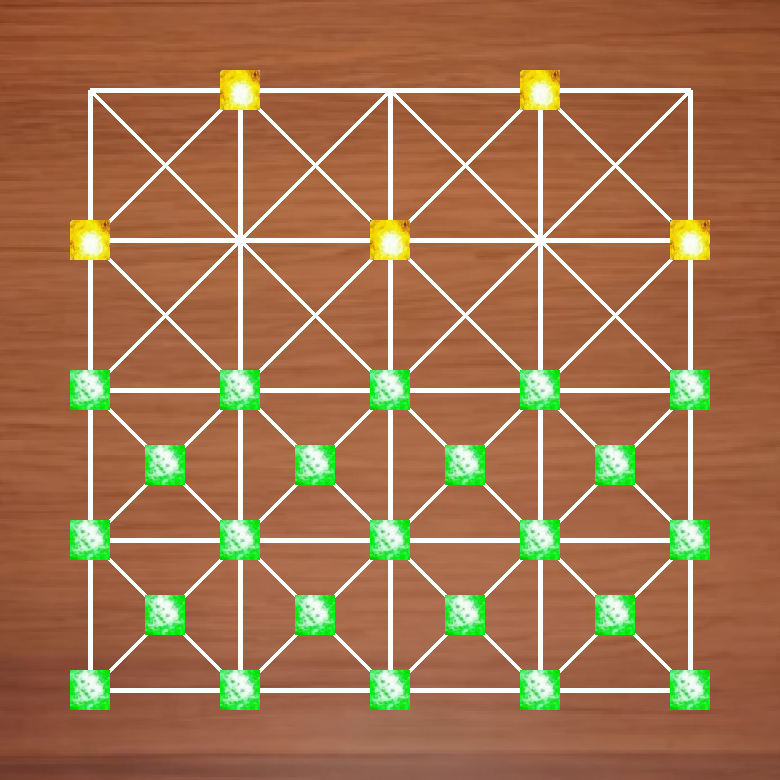
\includegraphics[height=4.2cm]{figures/end_blocked.png}
    \caption{Blockaded: Yellow still has 5 pieces but every landing cell is
    occupied or off the board (a reduced example).}
  \end{subfigure}
  \caption{The two ways to lose. The 2-player mode has no draws. A side that
  temporarily has no move while it is \emph{not} its turn has not yet
  lost---the condition is checked only at the start of its own turn.}
  \label{fig:endgame}
\end{figure}
